\section{Simulation Evaluation} \label{sec:simulation}

We have developed a simulation framework for comparing the \textsc{STAM} task scheduling to traditional scheduling algorithms.  Our simulation includes a stochastic energy harvesting process, a random task list and \textsc{STAM} task list generator, the scheduling processes, and an execution process.  We execute $n$ simulations on one task list per run, and generate task lists for $r$ runs.  Each task list consists of $k$ tasks.

\subsection{Task Generation}
The tasks are generated with random periods, durations, and energy requirements.  The periods and durations are distributed uniformly in discrete time steps measured in days, ranging respectively from 10 to 40 and from 1 to 4.  The energy is half-normally distributed, and proportional to the task's period (\emph{i.e.} a task requiring high energy is expected to run at a low frequency).

A random task list and its corresponding virtual task list generated by \textsc{STAM} are generated reiteratively until both lists are temporally schedulable.  We consider a task list temporally schedulable when its CPU utilization $U$ is less than 100\%.  The utilization is calculated with equation~\ref{eqn:utilization}, where $k$ is the number of tasks, $d_i$ is the duration of the $i^{th}$ task, and $p_i$ is the period of the $i^{th}$ task. [source]
\begin{equation}
\label{eqn:utilization}
U = \sum_{i=1}^{k} \frac{d_i}{p_i}
\end{equation}
\subsection{Energy Harvesting Model}
We use a simple model of a photovoltaic energy harvester as a stochastic energy source for our simulation.  The energy withdrawn from the environment is modeled as a 3-state Markov chain (\cite{poggi2000stochastic,moser2007real}) representing three weather conditions (figure~\ref{fig:markov}).  At each discrete time step during the simulation the Markov chain is updated, and the energy generated added to an energy pool (\emph{i.e.} a battery).
\begin{figure}[htb]
\label{fig:markov}
\caption{Markov Chain Weather Model.}
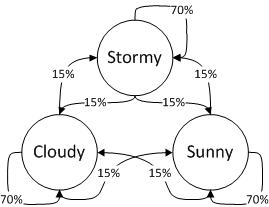
\includegraphics{markov.png}
\end{figure}
We generated a table of energy inputs to the system using the solar cell model that comes with Simulink's SimElectronics toolkit, configured with values from \cite{gonzalez2006model}.  

\begin{table}[h]
\begin{center}
\begin{tabular}{| l | l || l | l |}
\hline
\textbf{Rad. ($\frac{W}{m^2}$)} & \textbf{Charge ($A\cdot d$)} & \textbf{Rad. ($\frac{W}{m^2}$)} & \textbf{Charge ($A\cdot d$)} \\
\hline
50 & 0.190 & 175 & 0.665 \\
75 & 0.285 & 200 & 0.760 \\
100 & 0.380 & 225 & 0.855 \\
125 & 0.475 & 250 & 0.950 \\
150 & 0.570 & 275 & 1.045 \\
\hline
\end{tabular}
\end{center}
\label{tab:radiance}
\caption{Solar panel energy output}
\end{table}

We use the values of 50, 100, and 200 $\frac{W}{m^2}$ to represent the stormy, cloudy, and sunny weather conditions.

The output current of the photovoltaic cell, $I_c$, is governed by a two-diode formula given in \cite{marwali1997probabilistic} and modelled by the Simulink model.  The current flows into a battery, for which we use a linear model without relaxation effect.  The battery capacity at time $t$, $B_t$ is calculated using equation~\ref{eqn:batterycharge} per \cite{niyato2007sleep}.
\begin{equation}
 B_t = B_{t-1} + I_c \Delta t - I_d \Delta t
\label{eqn:batterycharge}
\end{equation}
where 
\begin{description}
\item[$B_{t-1}$] is the previous battery capacity
\item[$I_c$] is the charge current due to solar harvesting during $\Delta t$
\item[$I_d$] is the discharge current due to task execution during $\Delta t$
\end{description}
We represent $I_c$ and $I_d$  as constant averages during the interval $\Delta t$. Furthermore, the battery is
limited in capacity, such that if $B_t = B_{max}$ then any excess energy that is harvested is lost.

\subsection{Simulation Results}
We performed 1000 runs, with one run consisting of 100 simulations each on several task schedules using common random numbers (\emph{i.e.} using the same weather patterns).  Each simulation covered a 100-day period, and if the battery charge dropped to 0 during the simulation we incremented a violation counter.  We recorded the number of violations produced during each run.  Figure \ref{fig:violationhist} shows a histogram of violations that occurred during a simulation with our chosen parameters.
\begin{figure}[h]
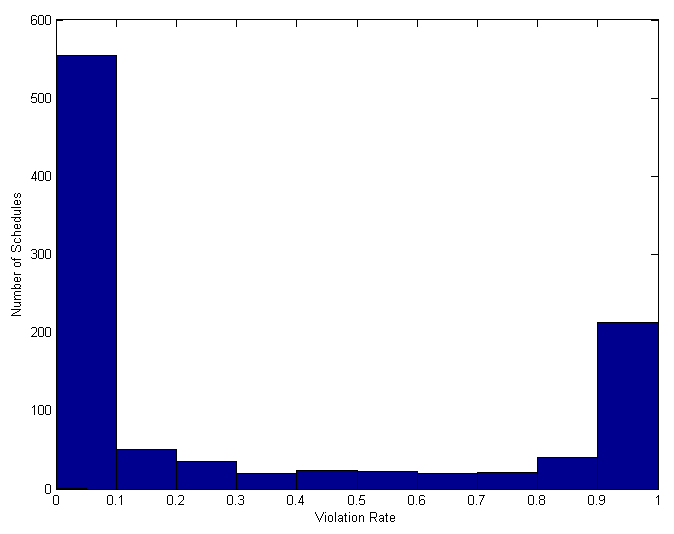
\includegraphics[scale=0.5]{violationhistogram.png}
\label{fig:violationhist}
\caption{Histogram of violation counts over 1000 runs.}
\end{figure}
Clearly most of the random task lists were easy to schedule without energy violations.  Many task lists were very difficult to schedule---presumably these correspond to task lists with tasks that take an abnormally large amount of energy and/or have a large duty cycle.

Compare results of EDF vs. STAM































